%\bibliographystyle{sjtu2}%[此处用于每章都生产参考文献]
\chapter{针对动态场景的学习索引系统:\sys}
\label{chap:sys}

面对动态场景下的挑战,包括动态数据分布带来的挑战与访问模式带来的挑战,
为了实现{\li}的最佳性能,我们提出了一个新的针对动态场景的学习索引系统{------}{\sys}。
{\sys}主要由三部分构成:\textbf{训练集生成器(Training Set Generator)}、\textbf{咨询器(Counselor)}和\textbf{终结器(Finalizer)},
它通过模型缓存机制来大幅减少动态数据分布下的{\rmi}架构搜索时间,通过数据数据拉伸方法来使{\li}的构建中考虑访问模式信息。

本节将首先介绍{\sys}的高层设计,随后分别介绍{\sys}各部件的具体设计。
为便于呈现,测试评估将与设计穿插在一起。

% To achieve learned indexes' best performance, we propose
% a new learned index system for dynamic workloads called \sys (\Cref{fig:sys}).
% \sys incorporates read access pattern using the \textbf{Training Set Generator} and the
% \textbf{Finalizer} and reuses pre-trained models using the \textbf{Counselor}.

\section{总览}

\begin{figure}[!ht]
  \centering
  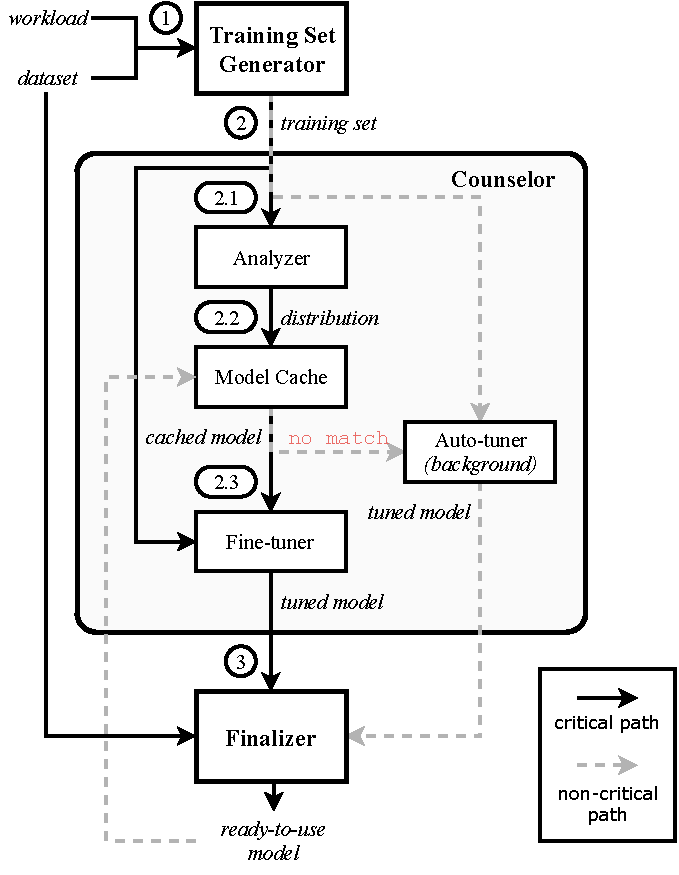
\includegraphics{figure/Doraemon.pdf}
  \bicaption[{\sys}架构示意图]
    {{\sys}架构示意图}
    {The illustration of \sys architecture}
  \label{fig:arch}
\end{figure}

图\ref{fig:arch}展示了{\sys}的架构设计。

系统每次运行时,工作负载信息和被索引的数据成作为系统输入,首先被训练集生成器接收。
训练集生成器从工作负载信息中抽取访问模式信息,并通过数据拉伸方法将访问模式信息与被索引的数据结合在一起,生成包含访问模式信息的新的训练集。
通过训练集生成器,我们可以做到不修改{\rmi}训练与推断算法的同时将其性能针对实时访问模式进行优化。
此外,目前训练集生成器仅提取访问模式信息,但针对其他动态负载下可以优化{\li}性能的信息均可在这一阶段被提取,这一方向的探索将会是未来的工作。

新生成的包含访问模式信息的新训练集随后被咨询器接收,由咨询器根据这一训练集生成较优
\footnote{我们不能使用“最优”一词因为在无穷的搜索空间且缺乏理论推导支撑下,我们不能断言某{\rmi}架构的“最优”性质。}
的{\rmi}架构与参数。
在咨询器内部,我们使用模型缓存机制,尽可能地重用已有的架构搜索结果,避免大量的枚举的架构搜索工作。
当缓存下来的{\rmi}架构与参数与当前输入训练集有较大出入时,我们异步地进行架构搜索工作,避免对索引性能的影响。

最后,终结器使用被索引的数据重新训练{\rmi}最后级{\model}的参数以及更新它们的误差值。
这是因为由训练集生成器产生的训练集仅用于训练中间级{\model}以获得更优的数据分配方式,而对于定位数据,我们仍需要在真实数据位置信息上训练最后级{\model}。

当{\sys}监测到数据分布或访问模式发生较大变化时,便会运行以上流程,在使用已有{\rmi}架构与参数进行服务的同时,寻求更优的{\rmi}架构与参数。
新的{\rmi}架构与参数与对应的数据分布和访问模式将会异步地被模型缓存记录下来,以便将来的重用。
目前,我们通过检测{\li}性能下降作为数据分布或访问模式发生较大变化的指标。

\section{训练集生成器}

训练集生成器首先需要从工作负载信息中抽取访问模式信息。
在目前的实现中,我们通过记录搜索键范围的访问频率。
具体的,我们将被索引的数据根据搜索键分为多个等长范围,给每个范围设置一个访问计数器,并在每次访问时记录更新计数器,从而获得通过访问频率表示的访问模式信息。
计数器在每次发生{\rmi}架构和参数的更新后会清零,以反应实时的访问模式。

数据集生成器从工作负载统计信息中的统计数据中获取访问模式信息后,将访问模式信息与被索引的数据结合在一起,生成包含访问模式信息的新的训练集,
并将生成的训练集发送给咨询器。
通过仅修改训练集,我们可以做到不修改{\rmi}训练与推断算法的同时将其性能针对实时访问模式进行优化。

% Training Set Generator takes the workload and dataset as
% input, extracts the access pattern by uniformly sampling
% from the workload and stretches the dataset according to the access
% pattern. Then it sends the stretched training set to Counselor
% to get a tuned model.

\subsection{一个直观的尝试}
\label{sec:pattern-intuitive}

训练集生成器的目的在于使{\li}的构建中能够考虑访问模式信息。
为了在{\li}的构建中考虑访问模式信息,一个直观的办法是在训练时加大{\hotkey}对训练结果的影响,
比如在随机梯度下降(stochastic gradient descent,SGD)中更多地使用{\hotkey}进行迭代训练。
因为根据这类算法,当某数据条目被反复作为训练数据执行训练算法时,针对优化这条数据下的精确度的参数更新将会发生更加频繁,从而导致这条数据具有更低的误差值。

为了实现这一点,我们尝试根据其访问频率复制{\hotkey},构成新的训练集。
假设一个训练集包含以下数据:$\{<a, 0>, <b, 1>, <c, 2>, <d, 3>\}$,其中每个对的第一个元素是键而第二个元素是该键对应的位置,
如果这三个键的访问频率是$1:2:2:1$,则我们复制键$b$和$c$的训练数据,得到以下新的训练集$\{<a, 0>, <b, 1>, <b, 1>, <c, 2>, <c, 2>, <d, 3>\}$。
通过这样,{\model}将会以两倍的概率被$<b, 1>$和$<c, 2>$训练,从而对键$b$和键$c$的预测准确度将会被提高。

% To incorporate read access pattern, an intuitive solution is to increase the
% contribution of frequently accessed keys during the training process.
% This can be achieved by creating multiple copies of those keys in the
% training set. For example, considering a training set of
% \{(a, 0), (b, 1), (c, 2)\}, where the first element is
% the key and the second is its position. If the accessed ratio is 1:2:1,
% then we double \emph{b} in the training set,
% which becomes \{(a, 0), (b, 1), (b, 1), (c, 2)\}.
% In this way, the model will be trained with (b, 1) two times more than others, the prediction
% accuracy of \emph{b} can be improved.

然而,这一直观的方法并非针对访问模式的最优解决方案,因为这一方法仍然依据原论文提出的均匀分配数据分配原则,
并且优化{\hotkey}的误差并不直接反映在对应的{\rmi}最后级{\model}的最大误差和最小误差。
针对这一情况,我们提出数据拉伸方法,一个创新性的方案将将访问模式信息与被索引的数据结合在一起,生成包含访问模式信息的新的训练集来优化{\rmi}中间级的数据分配策略。
使用数据拉伸,我们可以做到不修改{\rmi}训练与推断算法的同时将其性能针对实时访问模式进行优化。

\subsection{数据拉伸}

根据第\ref{sec:pattern-affect-li}节的分析,与其优化热键的预测误差,我们应该关注处理{\hotkey}{\model}的数据量。
因为被分配键数量较少的{\model}往往会拥有较小的误差范围,我们尝试使用数据拉伸的方法来减少处理{\hotkey}的{\model}所被分配的键的数量。

我们可以如此地直观理解数据拉伸{------}是{\rmi}最后级{\model}的数据量与这些数据被访问的频率负相关,搜索键越被频繁地访问则它们对应的{\rmi}最后级{\model}所索引地数据量越少。
具体的,对于{\hotkey},我们将增大其在训练集中与其他键的距离,即改变键所对应的数据位置的值,并用新的训练集来训练除了最后级之外的{\model},从而实现以上数据分配的效果。
因为中间级的{\model}会依据被拉伸后的训练集进行分配数据,而在新的训练集中{\hotkey}将以较少的数量占据较大的(拉伸后的)“{\cdf}”值域空间。
而我们未修改{\rmi}的训练和推断算法,因此数据会根据拉伸后的“{\cdf}”进行“均匀”分配,
从而最终在最后级分配的数据将会达到对于处理{\hotkey}的{\model}仅被分配少量数据的效果,
进而优化了最终{\hotkey}的查询性能。
这一方法成为“基准线方法”。

%     \begin{center}
%         \includegraphics[width=0.9\columnwidth]{figure/results/stretch.eps}
%     \end{center}
%     \caption{
%         \label{fig:stretch}
%         The left figure shows CDF of original D1, while the right figure shows CDF of D1 after stretched.
%     }
%     \end{figure}
%     %---------------------------
% \textbf{“Stretch” the dataset.} Instead of improving the prediction
% accuracy of the hot keys, we should focus on the error bounds
% of the models containing the hot keys (hot models). Since the models assigned with few keys tend to
% have small error bounds, we try to reduce the number of keys handled by
% the hot models by “stretching” the dataset.
% If a key is frequently accessed, we would like to increase
% the distance between it with its neighbors, the key before or
% after it. It can be achieved by simply shifting the position
% labels.

\begin{figure}[!htp]
  \centering
  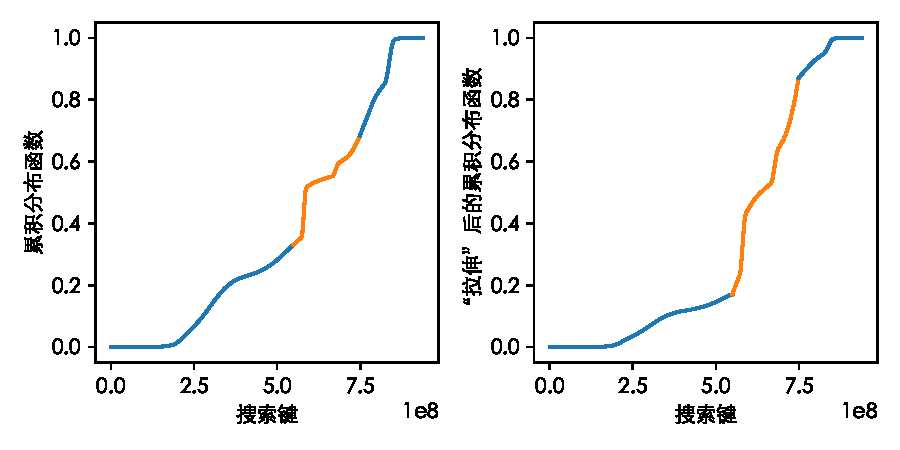
\includegraphics{figure/stretching.pdf}
  \bicaption[数据拉伸示意图]
    {数据拉伸示意图}
    {The illustration of Data Stretching}
  \label{fig:stretch-illus}
\end{figure}

具体地,对于给定键$key$,在新的训练集里该键对应的数据位置值为$F(key) \times N$,其中$F(key)$为从最小键到该键前的累计访问频率,$N$为总共键个数。
对于上文提到的例子,原训练集为$\{<a, 0>, <b, 1>, <c, 2>, <d, 3>\}$且这三个键的访问频率是$1:2:2:1$,
则在数据拉伸后的训练集为$\{<a, 0>, <b, 0.7>, <c, 2>, , <d, 3.3>\}$。
图\ref{fig:stretch-illus}直观地展示了针对第一个数据集(D1)在数据拉伸前后的训练集。
我们可以明显地看到,数据拉伸很好地将热点键在训练数据中分散开,从而使用新的训练集训练中间级{\model}进行数据分配能够很好地减少处理{\hotkey}的{\model}所被分配的键的数量。

% Specifically, given a key with position $p$ before “stretching”, if its access frequency is $f$, and the dataset size is $N$
% then we need to shift its position to be $p + (n-1)/2$, and shift
% all keys after it with $n-1$. For the above example, the training
% set of \{(a, 0), (b, 1), (c, 2)\} with access
% frequency 1:2:1 will be augmented to be \{(a, 0), (b, 1.5), (c, 3)\}. Figure~\ref{fig:stretch} shows the CDF of dataset 1
% before and after “stretching” with the access pattern in workload
% Skewed 3.

\subsection{训练集生成器效能测评与分析}

\begin{table}[!hpb]
  \centering
  \bicaption[不同解决访问模式挑战方法的性能评估]
    % {一个颇为标准的三线表格\footnotemark[1]}
    {不同解决访问模式挑战方法的性能评估}
    {Performance evaluation of different approaches handling access pattern}
  \label{tab:pattern-sol}
  \begin{tabular}{lccc}
  \toprule
                & 原始方法  & 基准线方法  & 数据拉伸  \\ \midrule
  吞吐量(MOPS)        & 3.54    & 3.47     & 6.37    \\
  误差范围  & 10.34     & 10.08     & 7.76     \\ \bottomrule
  \end{tabular}
\end{table}

我们使用第一个数据集(D1)在第三个{\skewwl}(Skewed 3)下比较了原始方法、第\ref{sec:pattern-intuitive}节提出的直观的方法与数据拉伸方法对{\li}性能的影响。
在表\ref{tab:pattern-sol}中,我们可以看到使用了直观的方法下新的训练集,最佳的{\rmi}架构是在第一层使用隐藏层宽度为16、隐藏层个数为1的{\nn}的{\rmi}架构,
其平均吞吐量为3.54 MOPS,和{\li}的性能(3.47 MOPS)非常接近。
事实上,这一结果是符合预期的,也与第\ref{sec:pattern-affect-li}节的分析相一致。
这是因为,这种直观的方法并不能优化{\model}的最大误差和最小误差,而是只能优化{\hotkey}的误差值,
然而{\model}的最大误差和最小误差才是决定{\li}性能的关键因素。
同时,在这一直观方法下,{\rmi}的中间级对数据的分配依然是尊重均匀分配原则的,这一直观方法只是让针对{\hotkey}的分配更加趋于均匀而已。
而根据第\ref{sec:pattern-affect-li}节的分析,针对{\hotkey},不均匀的分配反而会带来更好的性能。
我们可以看到,处理{\hotkey}的{\model}的平均误差并没有较好的提升,因此,这一直观方法并不能够在考虑访问模式信息下优化{\li}的性能。

% We evaluate this intuitive
% solution with the workload of Skewed 3 and the dataset D1. With the new
% training set, the best architecture we can find is NN16 with 275 ns average search time,
% which is close to the previous best architecture, 282 ns. This is because the intuitive solution does not
% improve the error bounds of the second stage models
% which decide the search time. In the above evaluation, the
% average error bound does not improve much (5.21 vs. 5.31).

另一方面,使用数据拉伸方法的{\li}拥有高于其他两种方法的性能表现,这是因为数据拉伸有效地将{\rmi}中间级{\model}地数据分配原则按照访问模式进行优化,
有效地减少处理{\hotkey}的{\model}的最大误差和最小误差,进而提高索引性能。
使用数据拉伸能够减少25.0\%模型误差范围,带来高达79.9\%的性能提升。

\begin{figure}[!htp]
  \centering
  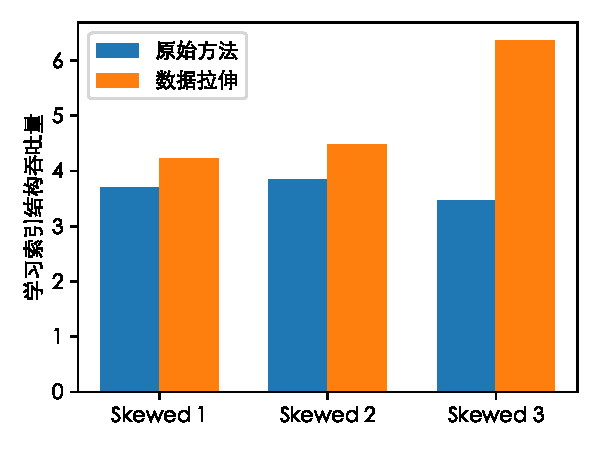
\includegraphics{figure/stretching-result.pdf}
  \bicaption[使用数据拉伸的{\li}在不同{\skewwl}下的性能表现]
    {使用数据拉伸的{\li}在不同{\skewwl}下的性能表现}
    {The learned index performance with Data Stretching under workloads with significant locality of reference}
  \label{fig:stretch-result}
\end{figure}

我们进一步在考虑更多地{\skewwl}下数据拉伸方法地有效性。
图\ref{fig:stretch-result}展示了在第一个数据集(D1)、不同{\skewwl}下{\li}的性能,我们可以看到,针对不同的{\skewwl}直观的方法对性能提升非常有限,
而数据拉伸能够有效地改进{\li}地索引性能。
通过实验我们验证了数据拉伸方法对广泛存在于真实场景中的访问模式有着较好地效果。

\section{咨询器与终结器}

通过训练集生成器,原始数据分布与访问模式信息同一在一个训练集中,因此我们只需要考虑在新的训练集下何种{\rmi}架构能够产生较优性能,具体的我们考虑新训练集的数据分布。
根据观察,对于类似的训练集数据分布,较优的{\rmi}架构也是类似的。
根据这一观察,对于类似的训练集数据分布,重复地进行架构搜索工作是多余的。
因此,{\sys}通过保留一个从训练集数据分布到过去训练的{\rmi}架构和参数的映射,来重用过去{\rmi}架构搜索的结果,
减少面对动态数据分布,为持续性保持{\li}优秀性能所需要的高昂架构搜索代价。

% After incorporating the access pattern, the only factor affecting
% the model architecture is data distribution.
% We notice that the best model architecture tends to be the same for similar data distributions.
% As a result, \sys is able to cache a mapping from data distributions to
% models for future reusing.

以上功能由咨询器提供,咨询器包括以下四部分:\textbf{分析器(Analyzer)}、\textbf{模型缓存(Model Cache)}\textbf{微调器(Fine-tuner)}和\textbf{自动调整器(Auto-tuner)}。
训练集首先通过分析器产生一个简单的训练集数据分布表示,这个训练集数据分布表示随后被用于模型缓存来寻找最近似的缓存条目,即过去训练好的{\rmi}架构和参数。
匹配的{\rmi}架构和参数会经过微调器针对当前训练集进行微调,以适应当前训练集数据分布,获得最佳性能,随后将微调后的{\rmi}架构和参数返回。
注意,在这一个流程中并不涉及架构搜索工作,是一个非常轻量级的流程。
当匹配的{\rmi}架构和参数所对应的训练集数据分布与输入的训练集数据分布相差较远时,自动调整期会在后台异步地进行架构搜索工作,

% This is done by the Counselor component, which includes
% four modules:

在使用咨询器返回的{\rmi}架构和参数前,{\sys}通过终结器重新训练{\rmi}最后一级的{\model},以保证最终使用的{\rmi}有最佳预测性能且提供正确的误差范围,
随后{\sys}使用该{\rmi}架构和参数服务用户请求。

\subsection{分析器}

\begin{figure}[!htp]
  \centering
  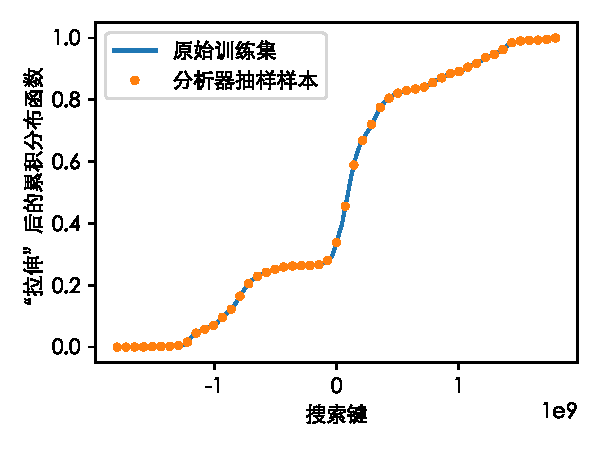
\includegraphics{figure/analyzer.pdf}
  \bicaption[分析器采样过程示意图]
    {分析器采样过程示意图}
    {The illustration of Analyzer's sampling process}
  \label{fig:analyzer}
\end{figure}

分析器对输入的训练集产生一个简单的训练集数据分布表示。
因为对于{\li}而言,训练集数据分布的关键在于{\cdf}的“形状”以及数据量大小。
对数据量大小信息而言,简单地用一个整型变量即可表示,因此不是咨询器的重点。
而如何表示{\cdf}的“形状”则对模型缓存的有效性非常关键。
因为{\cdf}的“形状”与数据量大小、搜索键的范围无关,因此我们选择通过抽样的方法进行训练集数据分布表示。
具体的我们从训练集中抽取$K$条样本来表示训练集数据分布信息,并将这些样本的键范围正则化到[0, 1]区间内。
图\ref{fig:analyzer}展示了分析器地工作流程。
$K$是一项可以调整的参数,它需要足够大来精确地表示训练集数据分布,但过大会给计算带来一定开销。

% \textbf{Analyzer:} extracts distribution information
% by uniformly sampling K records from the generated training set,
% then normalize both key and position to [0, 1]. However, K needs
% to be large enough to avoid
% breaking the distribution.

\subsection{模型缓存}

\begin{table}[!hpb]
  \centering
  \bicaption[不同训练集数据分布间的相似度度量]
    % {一个颇为标准的三线表格\footnotemark[1]}
    {不同训练集数据分布间的相似度度量}
    {The similarities between different datasets}
  \label{tab:similarity}
  \begin{tabular}{ccccc}
    \toprule
    \multirow{2}{*}{数据集1}  & \multicolumn{4}{c}{数据集2}              \\ \cmidrule{2-5}
                                & D1   & D2   & D3   & D4   \\ \midrule
    D1                          & 0  & 0.012  & 0.015  & 0.014  \\
    D2                          & 0.012  & 0  & 0.026  & 0.031  \\
    D3                          & 0.015  & 0.026  & 0  & 0.011  \\
    D4                          & 0.014  & 0.031  & 0.011  & 0  \\ \bottomrule
  \end{tabular}
\end{table}

模型缓存维护一个从训练集数据分布到过去曾经训练好的{\rmi}架构和参数,这个映射的键是由分析器产生的训练集数据分布表示。
目前由分析器产生的训练集数据分布表示是$K$个正则化的训练集数据采样序列,因此,我们通过以下公式计算两个采样序列的相似度度量:
\[
  similarity = \frac{ \sum_{i=1}^{K} (p_i - q_i)^2 }{ K }
\]
,其中$p_i$与$q_i$分别为采样序列$P$与$Q$的第$i$条数据采样。
相似度度量$similarity$越小说明两个训练集数据分布越接近。
表\ref{tab:similarity}展示了第\ref{sec:search-best}节中所用四个数据集间的相似度度量。
根据这一相似度度量,模型缓存能够快速地找到缓存中与输入训练集数据分布最接近地过去训练好的{\rmi}架构和参数。

% \textbf{Model cache:} maintains a mapping
% from the distribution of previous training set to their learning
% model's architure and parameters. If it receives a distribution
% from Analyzer,
% it will finds the entry in the map with the most similar
% distribution
% based on the mean square error. Then, it will send the model's
% information in that entry to Fine-tuner. Furthermore, if the
% similarity
% is below a threshold, it will also start the auto-tuning process.

\subsection{微调器}

微调器将在模型缓存中匹配的{\rmi}架构和参数用输入的训练集进一步进行微调,以适应当前训练集数据分布,获得最佳性能。
因为过去相似的训练集数据分布尽管与当前输入训练集数据分布类似,但在具体的函数映射上仍有细节上的出入,比如两者的搜索键范围可能有较大差异,
若不进行微调,{\rmi}中间级{\model}的数据分配可能会非常差。
因此,对模型缓存输出的{\rmi}架构和参数,微调器还会使用当前输入的训练集,增量式地对{\model}参数进行训练(incremental training)。
一个简单的增量式训练方法即将经典训练算法,比如随机梯度下降,的参数(权重)初始值设定为模型缓存输出的参数,从而在训练开始时,参数已能输出较为准确的预测结果,
从而降低微调训练时间。
经过微调后的{\rmi}架构和参数将作为咨询器的执行结果进行输出。

% \textbf{Fine-tuner:} incrementally trains the model retrieved from
% the model cache with the training set.

\subsection{自动调整器}

当输入咨询器的训练集数据分布与模型缓存中该分布最接近的数据分布间的相似度大于指定阈值时,
自动调整器将针对输入咨询器的训练集进行自动调整过程。
这是因为对于过去没有见过类似的训练集数据分布的情况下,没有保证模型缓存中的{\rmi}架构和参数能够在当前的训练集之下能够有较好的性能表现。
自动调整器将在预设的搜索空间内,使用网格搜索的方法来为输入咨询器的训练集找到最优的{\rmi}架构和参数。
自动调整过程在后台发生,不会阻塞任何索引查询操作。
自动调整过程结束后,获得的{\rmi}架构和参数将会被发送至终结器。

% \textbf{Auto-tuner:} uses grid search to find the best model architecture in the given search
% space.
% It performs auto-tuning at the background and sends the result to
% the Finalizer component.

\subsection{咨询器效能测评与分析}

\begin{table}[!hpb]
  \centering
  \bicaption[不同配置下咨询器运行时间]
    % {一个颇为标准的三线表格\footnotemark[1]}
    {不同配置下咨询器运行时间}
    {Counselor execution time with different configurations}
  \label{tab:counselor}
  \begin{tabular}{ccccccccc}
    \toprule
    \multirow{2}{*}{采样参数$K$}  & \multicolumn{8}{c}{模型缓存条目数目}                                                                        \\ \cmidrule{2-9}
                                 & \multicolumn{2}{c}{5k}  & \multicolumn{2}{c}{10k}  & \multicolumn{2}{c}{50k}  & \multicolumn{2}{c}{100k}  \\ \midrule
    100           & 0.40 s  & 0.067\%  & 0.41 s  & 0.068\%  & 0.50 s  & 0.083\%  & 0.61 s  & 0.102\%  \\
    500           & 0.43 s  & 0.072\%  & 0.44 s  & 0.073\%  & 0.54 s  & 0.090\%  & 0.69 s  & 0.115\%  \\
    1000          & 0.41 s  & 0.068\%  & 0.44 s  & 0.073\%  & 0.59 s  & 0.098\%  & 0.79 s  & 0.132\%  \\
    5000          & 0.46 s  & 0.077\%  & 0.50 s  & 0.083\%  & 0.83 s  & 0.138\%  & 1.25 s  & 0.208\%  \\ \bottomrule
  \end{tabular}
\end{table}

在上文的介绍中我们已经分别展示了咨询器各子组件的功效与性能分析,而咨询器的整体效能则体现在当训练集输入后,咨询器需要多少时间进行模型缓存的检索并返回微调后的结果。
表\ref{tab:counselor}展示了在不同采样参数$K$与模型缓存条目数目下咨询器完成其工作流程所需要的运行时间。
除了运行时间外,我们也给出了咨询器所需时间与没有咨询器的情况下使用网格搜索在有限架构搜索空间空间下进行最优架构搜索所需时间的比值。
我们可以清楚地看到咨询器的设置有效地缩短了动态数据分布下架构搜索的巨大代价。

\begin{figure}[!htp]
  \centering
  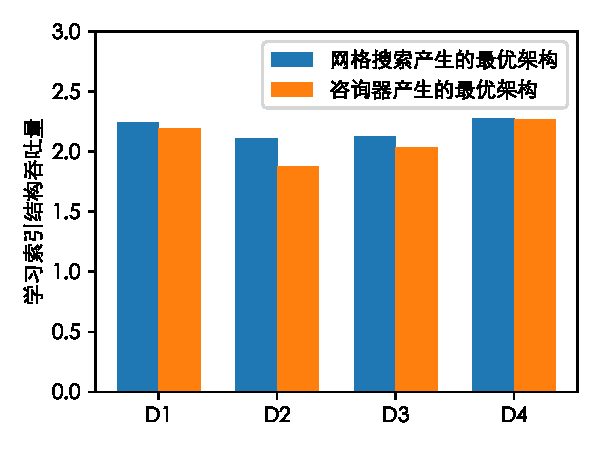
\includegraphics{figure/counselor.pdf}
  \bicaption[咨询器生成的{\li}架构性能表现]
    {咨询器生成的{\li}架构性能表现}
    {The learned index performance with Counselor-produced architectures}
  \label{fig::counselor}
\end{figure}

除时间节省外,我们也需要考虑模型缓存给出的最相似训练集数据分布下的{\rmi}架构与通过枚举方法得到的最优{\rmi}架构间性能差异。
图\ref{fig::counselor}展示了当模型缓存中仅存在第\ref{sec:search-best}节中所用四个数据集的历史信息下,对于任意一个数据集,
去除在模型缓存中其最优的{\rmi}配置后所产生的配置性能。
通过与通过枚举方法得到的最优{\rmi}架构间性能进行比较,我们看到通过模型缓存产生的{\rmi}配置性能与枚举下的最优性能差异非常小。
因此,尽管有时模型缓存产生的{\rmi}配置并非最优,但考虑其与枚举下的最优性能较小的差距以及其大幅节省的架构搜索时间,
我们认为模型缓存机制能够有效应对动态数据分布带来的挑战。

\subsection{终结器}

在使用咨询器返回的{\rmi}架构和参数前,终结器需要使用被索引的数据对应的{\cdf}(而非咨询器使用的由训练集生成器产生的训练集)重新训练{\rmi}最后一级的{\model}。
这是因为生成的训练集反应的并不是真实的数据位置,而是一个我们期望的中间级{\model}进行数据分配所遵循的分布。
对于{\rmi}最后一级{\model},我们仍然需要使用真实的数据位置来训练这些{\model},以保证这些用于输出对真实数据位置预测的{\model}有较为准确的预测,
并且保证这些{\model}记录的最大误差与最小误差能够用于提供二分搜索范围。
针对{\rmi}最后级{\model}的重训练过程往往很迅速,因为最后一级的往往是非常易于训练的{\lr},而使用1千条数据来训练{\lr}只需要118 $\mu$s。

经过终结器,我们的到了一个可以在当前数据分布与访问模式下提供良好性能的{\li}架构和参数。
在这一步之后,{\sys}便使用该{\li}架构和参数进行服务,同时将其加入到模型缓存中。

% Before using the returned model from Counselor, the Finalizer
% needs to retrain the last stage models with the original dataset.
% This is because the position of each key in the stretched training
% set is changed, we need to repair the position information
% with the original dataset. This process is considerably
% fast as last models are usually linear models. For example,
% it only takes 118 $\mu$s to retrain one last model with 1000 keys.

\subsection{终结器效能测评与分析}

\begin{table}[!hpb]
  \centering
  \bicaption[不同配置下终结器运行时间]
    % {一个颇为标准的三线表格\footnotemark[1]}
    {不同配置下终结器运行时间}
    {Finalizer execution time with different configurations}
  \label{tab:finalizer}
  \begin{tabular}{ccccc}
    \toprule
    \multirow{2}{*}{数据量大小}  & \multicolumn{4}{c}{{\rmi}最后级{\model}个数}                                           \\ \cmidrule{2-5}
                                & 10k  & 50k  & 100k  & 500k \\ \midrule
    10M           & 0.24 s   & 0.33 s  & 0.42 s  &1.23 s  \\
    50M           & 0.33 s   & 1.21 s  & 1.28 s  &2.36 s  \\
    100M          & 0.42 s   & 1.27 s  & 2.32 s  &3.63 s  \\
    500M          & 1.20 s   & 2.10 s  & 3.15 s  &11.50 s  \\
    1B         & 2.18 s   & 3.10 s  & 4.32 s  &12.76 s  \\ \bottomrule
  \end{tabular}
\end{table}

表\ref{tab:finalizer}展示了针对不同{\rmi}最后级{\model}个数、不同数据量下所需的训练时间。
同时我们也展示了这一时间占{\sys}所需总时间的比例。
我们可以看到,尽管终结器需要将{\rmi}最后级{\model}全部训练一次,但对总体时间的贡献并不大。
因此,我们认为终结器能够高效地协助{\sys}应对动态数据分布与访问模式带来的挑战。

\section{系统局限性}

\subsection{检测数据分布与访问模式的改变}

{\sys}在发现数据分布与访问模式发生改变的时候将执行以上描述的过程。
对数据分布与访问模式的改变的检测必须要即时,并且要求极小的误报(假阳性)率。
对于当前的设计,我们通过检测性能下降来表示数据分布与访问模式的改变。
在将来的工作中,我们可以使用类似\cite{kang2017noscope}的方法来提高检测数据分布与访问模式的改变的准确率。

% \textbf{Detecting the change of distribution and access pattern.}
% {\sys} will start to run on detecting the change of distribution or
% access pattern. The detection must be timely with few false positive.
% For currently design, we simply detect this by monitoring the
% degradation of the peformance. However, we can use similar technique
% in~\cite{kang2017noscope} to improve the accuracy.

\subsection{从数据集中提取数据分布}
当前,我们通过采样的方法来提取数据分布信息。
为了准确地表示分布信息,采样率,即参数$K$,需要进行精细地调整,给系统的实用性带来一定挑战。
我们期待在未来的工作中通过启发式或者基于机器学习的方法对该参数进行动态选择。

% \textbf{Extract the distribution feature from a dataset.} Currently, we
% simply extract the distribution by uniformly sampling the dataset.
% However, to avoid breaking the distribution, the sample rate varies
% across different dataset. As a result, it is challengin the decide the
% sample rate.

\subsection{相似度表示与计算}
我们对训练集数据分布的采样数据可以看作是一种序列数据,这一类数据在机器学习研究中被广泛地研究,存在着一系列针对此类数据的{\model}\cite{krizhevsky2012imagenet, szegedy2015going, simonyan2014very}。
我们相信进一步利用机器学习可以更好地获得相似度度量值,比如使用循环神经网络学习训练集数据分布的一个潜在表示(latent representation)并以此作为{\model}来判断两个训练集数据分布的相似度。
除此之外,统计学中的关于距离(distance)的研究也能够给相似度表示与计算提供借鉴,如相对熵(Kullback–Leibler divergence)。

% \textbf{Compute the similarity.}
% Our sampled distribution representation can be regarded as a type of sequential
% data, for which there are many machine learning models are targeting
% \cite{greff2017lstm, cho2014learning}.
% We believe we can further leverage learning to learn a better similarity metric.

\subsection{高效地计算与比较训练集数据分布}
模型缓存中可以存在大量缓存的训练集数据分布下的{\rmi}架构和参数,因此从中寻找相似的条目可能成为一件代价非常巨大的任务
,因为在当前的设计中我们需要与每一个缓存的训练集数据分布进行相似度计算与比较。
针对这一问题,我们计划在将来的工作中使用类似\cite{metwally2005efficient, ilyas2008survey}的方法滤最可能相似的条目,进而再进行精准地相似度匹配工作,从而提高相似度计算与比较的效率。

% \textbf{Efficiently find the similar distribution in Model Cache.} There can be
% throusands to millions entires in the Model Cache. As a result,
% finding the entry with most similar distribution is considerably
% cost. To solve this issue, we plan to use methods like
% \cite{metwally2005efficient, ilyas2008survey} to first filter out the most relevant
% entries before the comparison.

\subsection{优化自动调整器效能}
网格搜索非常缓慢。
为了提高搜索的速度,我们可以进一步利用高斯超参数优化\cite{snoek2012practical, bergstra2011algorithms, brochu2010tutorial}等启发式的自动参数调整算法来来加速自动调整器的架构搜索效能。
类似的想法已经在数据库优化中被使用\cite{duan2009tuning, thummala2010ituned}。
另一方面,自动机器学习领域的研究也可以应用在{\rmi}的架构搜索任务中。
这些探究将作为未来的工作。

% \textbf{Improve Auto-tuner efficiency.}
% Grid search is slow.
% To speed up the search, there are works that use Gaussian process to optimize
% the search process \cite{snoek2012practical, bergstra2011algorithms, brochu2010tutorial}.
% Similar ideas are also used in database system optimization \cite{duan2009tuning, thummala2010ituned}.